%CLASSE DOCUMENTO - LINGUA E DIMENSIONE FONT
\documentclass[11pt]{toptesi}

%%%%%%%%%%%%%%%%%%%%%%%%%%%%%%%%%%%%%%%%%%%%%%%%%%%%%%%%%%%%%%%

% INCLUSIONE PACCHETTI
		
%s\usepackage{fullpage}	
\usepackage{graphicx}
\usepackage[pagestyles]{titlesec}
\usepackage[flushleft]{caption}
\usepackage{setspace}
\usepackage[utf8]{inputenc} %utf8 % lettere accentate da tastiera
\usepackage[italian]{babel} % lingua del documento
\usepackage[T1]{fontenc} % codifica dei font
\usepackage{blindtext}
\usepackage{graphicx,wrapfig}
\usepackage{booktabs}
\usepackage{lmodern}
\usepackage{varioref}
\usepackage{url}
\usepackage{array}
\usepackage{paralist}{\obeyspaces\global\let =\space}
\usepackage{verbatim} 
\usepackage{subfig}
\usepackage{tabularx}
\usepackage{amsmath}
\usepackage{amsfonts}
\usepackage{float}
\usepackage{amssymb}
\usepackage{multicol}
\usepackage{multirow}
\usepackage{listings}
\usepackage[pass]{geometry}
\usepackage[figuresright]{rotating}
\usepackage{algorithm}
\usepackage{algorithmic}
\usepackage{amsmath}
\usepackage[babel]{csquotes}
\usepackage{hyperref}
\usepackage[backend=bibtex]{biblatex}

%%%%%%%%%%%%%%%%%%%%%%%%%%%%%%%%%%%%%%%%%%%%%%%%%%%%%%%%%%%%%%%

% CONFIGURAZIONE LINK E RIFERIMENTI
\hypersetup{%
    pdfpagemode={UseOutlines},
    bookmarksopen,
    pdfstartview={FitH},
    colorlinks,
    linkcolor={black}, %COLORE DEI RIFERIMENTI AL TESTO
    citecolor={blue}, %COLORE DEI RIFERIMENTI ALLE CITAZIONI
    urlcolor={blue} %COLORI DEGLI URL
}

%%%%%%%%%%%%%%%%%%%%%%%%%%%%%%%%%%%%%%%%%%%%%%%%%%%%%%%%%%%%%%%

% CONFIGURAZIONE LISTATI/CODICE - CANCELLARE SE NON NECESSARIO
% PYTHON - BIANCO E NERO
\lstset{%
	captionpos=b,
	language=Python,
	basicstyle =\small\ttfamily,
	keywordstyle=\color{black}\bfseries,
	breaklines=true,
	breakatwhitespace=true,
	frame=lines,
	numbers=left,
	numberstyle=\footnotesize,
}

%%%%%%%%%%%%%%%%%%%%%%%%%%%%%%%%%%%%%%%%%%%%%%%%%%%%%%%%%%%%%%%

% FRENCHSPACING VA _SEMPRE_ ABILITATO PER DOCUMENTI IN ITALIANO
\frenchspacing

%%%%%%%%%%%%%%%%%%%%%%%%%%%%%%%%%%%%%%%%%%%%%%%%%%%%%%%%%%%%%%%

%DEFINIZIONE SEZIONI IN NUMERAZIONE ROMANA
%ELENCO DEI LISTATI/CODICI
\makeatletter
\newcommand\listofcodes{%
 \iffrontmatter\else\frontmattertrue\fi
 \if@openright\cleardoublepage\else\clearpage\fi
 % change the meaning of \chapter in a group
 \begingroup\def\chapter##1{\@schapter}
 \phantomsection % for the hyperlink
 \lstlistoflistings 
 \endgroup
} 
\makeatother

%%%%%%%%%%%%%%%%%%%%%%%%%%%%%%%%%%%%%%%%%%%%%%%%%%%%%%%%%%%%%%%

% INFORMAZIONI PDF - PERSONALIZZARE
\pdfinfo{%
  /Title    (Apprendimento della personalità basato sul linguaggio naturale)
  /Author   (Giorgia Adorni)
  /Subject  (Laura Informatica)
  /Keywords (Tesi)
}

%%%%%%%%%%%%%%%%%%%%%%%%%%%%%%%%%%%%%%%%%%%%%%%%%%%%%%%%%%%%%%%


% LISTA DEI CAPITOLI DA INCLUDERE - PERSONALIZZARE
\includeonly{%
frontespizio,%
abstract,%
introduzione,%
neural_network,%
chap_quo,%
chap_qua,%
app_a,%
}

%%%%%%%%%%%%%%%%%%%%%%%%%%%%%%%%%%%%%%%%%%%%%%%%%%%%%%%%%%%%%%%


% FILE DI BIBLIOGRAFIA
\bibliography{bibliography} 

% INIZIO DOCUMENTO
\begin{document}
	
% FRONTESPIZIO
\newpage
\pagestyle{empty} % no number
\noindent

\begin{figure}\doublespacing
	\mbox{
				\begin{minipage}{.20\textwidth}
					\includegraphics[height=3.3cm]{images/LogoBicocca.pdf}
				\end{minipage}%
				\quad\quad
				\begin{minipage}[c]{.90\textwidth}
					{Università degli Studi Milano Bicocca}\\
					{  \textbf{Scuola di Scienze}}\\
					{\textbf{Dipartimento di Informatica, Sistemistica e Comunicazione}}\\
					{  \textbf{Corso di Laurea in Informatica}}
				\end{minipage}%
	}

\end{figure}

\begin{center}
	\vspace{35mm}
\doublespacing\textbf{\huge RETI NEURALI PER~L’APPRENDIMENTO DEI TRATTI DELLA PERSONALITÀ DAL LINGUAGGIO NATURALE }\\
	
\end{center}

\vspace{30mm}
\onehalfspacing 

\begin{tabular}{ll}
	\textbf{Relatore: } & {Prof. Stella Fabio Antonio}\\
	\textbf{Co-relatore: } & {Dott. Marelli Marco}
\end{tabular}

\vspace{5mm}

\begin{flushright}\onehalfspacing 
	\textbf{Relazione della prova finale di:}\\
	{Giorgia Adorni}\\
	{Matricola 806787}\end{flushright}

\vspace{25mm}
\begin{center} \textbf{Anno Accademico 2017-2018 }\end{center}


%%%%%%%%%%%%%%%%%%%%%%%%%%%%%%%%%%%%%%%%%%%%%%%%%%%%%%%%%%%%%%%

%INTERLINEA - DEFAULT 1 - NON ESAGERATE, NON SUPERATE MAI 1.3 ;)
%\interlinea{1.2}

%%%%%%%%%%%%%%%%%%%%%%%%%%%%%%%%%%%%%%%%%%%%%%%%%%%%%%%%%%%%%%%
\frontmatter

% DEDICA
% VSPACE - PROPORZIONE USATA PER CENTRATURA VERTICALE DEL TESTO
% FLUSHRIGHT - ALLINEAMENTO ORIZZONTALE A DESTRA
\vspace*{\stretch{1}}
\begin{flushright}
\noindent
\textit{A mio padre. }\\
\textit{Al mio fidanzato e collega. }
\end{flushright}
\vspace*{\stretch{6}}
\cleardoublepage


% CITAZIONE 
% VSPACE - PROPORZIONE USATA PER CENTRATURA VERTICALE DEL TESTO
% FLUSHRIGHT - ALLINEAMENTO ORIZZONTALE A DESTRA
\vspace*{\stretch{1}}
\begin{flushright}
\noindent
Citatemi dicendo che sono stato citato male.

\textit{Groucho Marx}
\end{flushright}
\vspace*{\stretch{6}}
\cleardoublepage

%%%%%%%%%%%%%%%%%%%%%%%%%%%%%%%%%%%%%%%%%%%%%%%%%%%%%%%%%%%%%%%

% RINGRAZIAMENTI - PERSONALIZZARE
\ringraziamenti
Grazie al mio relatore Fabio Stella e ai ragazzi del laboratorio MAD (Models and Algorithms for Data \& text mining).

%%%%%%%%%%%%%%%%%%%%%%%%%%%%%%%%%%%%%%%%%%%%%%%%%%%%%%%%%%%%%%%

% ABSTRACT - PERSONALIZZARE
\sommario

La personalità è considerata come uno degli argomenti di ricerca più influenti in psicologia poiché predittiva di molti esiti consequenziali come la salute mentale e fisica, ed è in grado di spiegare il comportamento umano.
Grazie alla diffusione dei Social Network come mezzo di comunicazione, sta diventando sempre più importante sviluppare modelli che possano leggere automaticamente e con precisione l'essenza di individui basandosi esclusivamente sulla scrittura. 
\\\\
In particolare la convergenza tra scienze sociali e informatiche ha portato i ricercatori a sviluppare approcci automatici per estrarre e studiare le informazioni "nascoste" nei dati testuali presenti in rete.
La natura di questo progetto di tesi è altamente sperimentale, e la motivazione alla base di questo lavoro è presentare delle analisi dettagliate sull'argomento, in quanto allo stato attuale non esistono importanti indagini di questo tipo.
\\\\
Obiettivo è identificare un adeguato spazio semantico che permetta di definire la personalità dell'oggetto a cui un determinato testo si riferisce. Punto di partenza è un dizionario di aggettivi che la letteratura psicologica definisce come marker dei cinque grandi tratti di personalità o Big Five.
\\\\
In questo lavoro siamo partiti dall'implementazione di reti neurali  fully-connected come base per capire come i modelli semplici in deep-learning possano fornire informazioni sulle caratteristiche della personalità nascoste. 
\\\\
Infine utilizziamo una classe di algoritmi distribuzionali inventati nel 2013 da \emph{Tomas Mikolov}, che consistono nell'utilizzo di una rete neurale convoluzionale, che impara in modo non supervisionato i contesti delle parole.
In questo modo costruiamo un embedding in cui sono contenute le informazioni semantiche del testo, ottenendo una sorta di “geometria del significato” in cui i concetti sono tradotti in relazioni lineari.
Con quest'ultimo esperimento ipotizziamo che uno stile di scrittura individuale sia in gran parte accoppiato con i tratti della sua personalità.

%%%%%%%%%%%%%%%%%%%%%%%%%%%%%%%%%%%%%%%%%%%%%%%%%%%%%%%%%%%%%%%

% INDICI 

% INDICE GENERALE
\tableofcontents

% INDICE DELLE FIGURE
\listoffigures

% INDICE DELLE TABELLE
\listoftables

% INDICE DEI CODICI
\listofcodes

%%%%%%%%%%%%%%%%%%%%%%%%%%%%%%%%%%%%%%%%%%%%%%%%%%%%%%%%%%%%%%%
\mainmatter

% INCLUSIONE FILE CAPITOLI - TENERE COERENTE CON LISTA IN ALTO
\chapter{Introduzione}
\label{chap:introduzione}
\Blindtext

Data mining: estrazione di significato da grandi quantità di dati
analisi dell'espressione umana che rendo conto da una parte del linguaggio come veicolo di definizione e di affermazione del se
evoluzione della comunicazione verso le nuove forme di dialogo tra persone e comunità

la raccolta di dadi e la necessità di produrre analisi sempre più velocemente ha fatto crescere in questa direzione la ricerca nel campo dell'apprendimento automatico o \emph{machine learning}.
In particolare, nell'ambito del text mining, si sono sviluppate metodologie che consentono ai computer di confrontarsi con il linguaggio umano, di elaborarlo e comprenderlo.


L'obiettivo di questa tesi è descrivere e sfruttare alcune tecniche come il machine learning e Natural Language Processing nell'ambito del ... 


Extroversion was the strongest predictor of leadership emergence — who becomes a leader — and leadership effectiveness — who's successful in a leadership position. But it was a better predictor of emergence than effectiveness.

What's more, when the study authors deconstructed extroversion into distinct parts, they found that dominance and sociability better predicted leadership than extroversion as a whole. This makes sense, the study authors write, "as both sociable and dominant people are more likely to assert themselves in group situations."
Conscientiousness, or a person's tendency to be organized and hard-working, was the second strongest predictor of leadership.
Again, conscientiousness was more closely linked to leader emergence than to leadership effectiveness. The authors write: "[T]he organizing activities of conscientious individuals (e.g. note taking, facilitating processes) may allow such individuals to quickly emerge as leaders.

In business settings, openness to experience is an important predictor of leadership. Justin Sullivan / Getty
Openness to experience was the third strongest predictor of leadership. However, it's worth noting that, in business settings specifically, openness was just as strongly linked to leadership as extroversion.
Neuroticism was not a strong predictor of leadership, meaning that highly neurotic people are not especially likely or unlikely to become leaders.
Agreeableness, or friendliness, was the "least relevant" to leadership of all the traits studied. Interestingly, however, when the researchers looked only at leadership effectiveness, agreeableness was related.




Psicologia e informatica:
I modelli computazionali possono essere utilizzati per modellare i sistemi come una scatola nera, ma possono anche essere usati per informare i modelli di elaborazione delle informazioni che mirano a comprendere la cognizione umana.




Le regioni cerebrali che codificano per vari tratti di personalità sono spesso accoppiate con regioni responsabili della comunicazione verbale e scritta. Inoltre, l'avvento dei social media e una comunità online sempre più connessa rendono sempre più disponibili i dati testuali personalizzati. In questo studio, ipotizziamo che uno stile di scrittura individuale è in gran parte accoppiato con i tratti della sua personalità e presenta un modello di apprendimento profondo per predire il tipo di personalità di Myers Briggs attraverso i dati testuali dei libri. Sviluppare un modello accurato e aprire questa domanda di ricerca avrebbe implicazioni significative nella business intelligence, nell'analisi della compatibilità delle relazioni e in altri campi della sociologia.










\chapter*{Abstract}
\label{Abstract}


Apprendimento della personalità basato sul linguaggio naturale. 
Reti neurali per la previsione dei tipi di personalità di Myers Brigg dagli stili di scrittura.






La personalità è l'essenza che definisce un individuo in quanto guida il modo in cui pensiamo, agiamo e interpretiamo stimoli esterni. 
Nel corso del secolo scorso, gli aspetti della personalità sono stati studiati da molti punti di vista, sia attraverso l'analisi delle relazioni interpersonali, delle dinamiche di gruppo e dei social network, sia attraverso le opere nelle neuroscienze che rivelano le basi biologiche dei tratti della personalità.


Il testo e la scrittura sono diventati un mezzo di comunicazione importante nell'era digitale. L'uso crescente dei social media e il fenomeno delle recensioni online hanno favorito un rapido aumento dei dati testuali digitali su cui vengono effettuate svariati tipi di analisi.
In particolare la convergenza tra scienze sociali (psicologiche) e informatiche hanno portato i ricercatori a sviluppare metodi automatizzati (approcci automatici) per estrarre e studiare le informazioni digitali contenute nel materiale testuale per prevedere i tratti della personalità.
La maggior parte degli attuali studi automatici di rilevamento della personalità si sono concentrati sul modello di personalità Big 5 come quadro per studiare le caratteristiche intrinseche dell'essere umano. 


Partendo da un dizionario di aggettivi che la letteratura psicologica definisce come marker dei cinque grandi tratti di personalità (Big Five), si vuole identificare un adeguato spazio semantico che permetta di definire la personalità dell’oggetto target a cui un determinato testo si riferisce. I dati che verranno utilizzati per definire lo spazio semantico e testare la sua funzionalità sono messi a disposizione da Yelp Dataset Challenge, che contiene 5˙200˙000 reviews relative a 174˙000 businesses di 11 aree metropolitane nel mondo. 




Obiettivo è la progettazione e lo sviluppo di un modello computazionale per l'apprendimento della personalità a partire dal linguaggio naturale.  


In questo studio, ipotizziamo che uno stile di scrittura individuale è in gran parte accoppiato con i tratti della sua personalità e presenta un modello di apprendimento profondo per predire il tipo di personalità di Myers Briggs attraverso i dati testuali dei libri. Sviluppare un modello accurato e aprire questa domanda di ricerca avrebbe implicazioni significative nella business intelligence, nell'analisi della compatibilità delle relazioni e in altri campi della sociologia.



La personalità è considerata uno degli argomenti di ricerca più influenti in psicologia perché è predittiva di molti esiti consequenziali come la salute mentale e fisica, la qualità delle relazioni interpersonali, l'adeguamento alla carriera e la soddisfazione, le prestazioni sul posto di lavoro e il benessere generale.

È ampiamente noto che i tratti della personalità come l'extraversione, la coscienziosità e il nevroticismo sono relativamente coerenti per tutta la vita. Tuttavia, i modi in cui i nostri comportamenti sono espressi attraverso le parole e l'azione non sono sempre determinati dai tratti soggettivi della personalità e dagli impulsi da soli.

Molte decisioni importanti, le dinamiche sociali e le decisioni politiche si basano anche sulla valutazione della personalità di un individuo con il quale non si è interagito molto personalmente. 

Ma leggere solo i comportamenti di altre persone non è sufficiente per fare previsioni accurate della loro personalità. Il compito diventa ancora più difficile quando si tenta di formulare giudizi basati solo sulla comunicazione scritta. 

Poiché il mondo si basa molto più sulla comunicazione basata sul testo rispetto alle interazioni faccia a faccia, sta diventando sempre più importante sviluppare modelli che possano leggere automaticamente e con precisione l'essenza di altri individui basandosi esclusivamente sulla scrittura. 

Fortunatamente, studi in neuroscienza hanno rivelato una mappatura vicina delle regioni del cervello responsabili dei tratti della personalità come l'extraversione e il nevroticismo, nonché quelli che sono legati alla comunicazione scritta.

I precedenti modelli di previsione della personalità si sono concentrati sull'applicazione di tecniche generali di apprendimento automatico e reti neurali per predire i tratti di personalità del Big Five di openness, conscientiousness, extraversion, agreeableness e neuroticism dai post sui social media. 

Gli studi che si focalizzano sui tratti del Big Five tendono a dare un tratto alla figura di un individuo.


In questo lavoro, abbiamo esplorato una varietà di metodi per affrontare il problema della predizione della personalità. 

Abbiamo iniziato costruendo manualmente un vasto corpus di brani tratti da romanzi famosi con autori di tipi MBTI. 

Per valutare la difficoltà di identificare gli MBTI dal testo, abbiamo raggruppato segmenti di testo basati su somiglianze di incorporamento di parole per determinare se esistesse una distribuzione non uniforme di tipi di personalità. Ciò fornisce una buona cornice iniziale di riferimento per capire quanto siano sottili i tratti della personalità quando sono nascosti nei dati scritti. 

Abbiamo poi implementato un sacco di reti neurali feed-forward come base per capire come i modelli semplici in deep-learning possano fornire informazioni sulle caratteristiche della personalità nascoste. 

Infine, ci addentriamo in una rete neuronale ricorrente basata sulla memoria a lungo termine più complessa e miriamo a costruire un sistema più generalizzabile che possa incorporare il significato della scrittura per determinare i tipi di personalità generali.



tratti di personalità Big 5.

I risultati delle analisi mostrano che il potere predittivo delle impronte digitali sui tratti della personalità è in linea con il 
Nel complesso, i nostri risultati indicano che la precisione delle previsioni è coerente tra i tratti Big 5 e che l'accuratezza migliora quando le analisi includono dati demografici e diversi tipi di impronte digitali.



struttura di personalità per guidare la nostra comprensione e rivelare il ruolo delle parole nel descrivere le caratteristiche di un utente. 
Questo studio preliminare ha rivelato come le percezioni del pubblico riguardo a parole specifiche possano aiutarci a rilevare la personalità. 

Come prima fase del nostro studio, questo esperimento si concentra sulla raccolta delle percezioni generali dei malesi verso 52 aggettivi inglesi categorizzazione delle parole sotto tratti PEN. 
La valutazione fornisce l'analisi necessaria che potrebbe aiutare la nostra ricerca principale che si concentra su rilevazioni automatiche della personalità. 










Abbiamo iniziato costruendo manualmente un vasto corpus di brani tratti da romanzi famosi con autori di tipi MBTI. 

Per valutare la difficoltà di identificare gli MBTI dal testo, abbiamo raggruppato segmenti di testo basati su somiglianze di incorporamento di parole per determinare se esistesse una distribuzione non uniforme di tipi di personalità. Ciò fornisce una buona cornice iniziale di riferimento per capire quanto siano sottili i tratti della personalità quando sono nascosti nei dati scritti. 



I risultati delle analisi mostrano che il potere predittivo delle impronte digitali sui tratti della personalità è in linea con il 
Nel complesso, i nostri risultati indicano che la precisione delle previsioni è coerente tra i tratti Big 5 e che l'accuratezza migliora quando le analisi includono dati demografici e diversi tipi di impronte digitali.


struttura di personalità per guidare la nostra comprensione e rivelare il ruolo delle parole nel descrivere le caratteristiche di un utente. 
Questo studio preliminare ha rivelato come le percezioni del pubblico riguardo a parole specifiche possano aiutarci a rilevare la personalità. 

Come prima fase del nostro studio, questo esperimento si concentra sulla raccolta delle percezioni generali dei malesi verso 52 aggettivi inglesi categorizzazione delle parole sotto tratti PEN. 
La valutazione fornisce l'analisi necessaria che potrebbe aiutare la nostra ricerca principale che si concentra su rilevazioni automatiche della personalità. 





\chapter{Reti Neurali}
\label{chap:RetiNeurali}

Nel campo dell'apprendimento automatico, o \emph{machine learning}, una rete neurale artificiale  in inglese \emph{Artificial Neural Network} (ANN),  è un modello matematico basato sulla semplificazione delle reti neurali biologiche \cite{samuel1959some}.

Una rete neurale può essere considerata come un sistema dinamico avente la topologia di un grafo orientato, i cui nodi modellano i neuroni in un cervello biologico, mentre gli archi rappresentano le sinapsi (interconnessioni di informazioni).

Ogni connessione può trasmettere un segnale da un neurone artificiale a un altro, i quali sono tipicamente aggregati in strati. Gli stimoli vengono ricevuti da un livello di nodi d'ingresso, detto unità di elaborazione, che elabora il segnale e lo trasmette ad altri neuroni ad esso collegati.

\section{Modello}
\label{sec:modello}

Le reti neurali possono essere viste come semplici modelli matematici che definiscono una funzione $f:X\rightarrow Y$. 

La funzione di rete di un neurone $f(x)$ è definita come una composizione di altre funzioni $g_i(x)$, che possono a loro volta essere scomposte in altre funzioni.

Una rappresentazione ampiamente utilizzata per la descrizione di ANN tradizionali è la \emph{somma ponderata}, mostrata nell'equazione \ref{eq:modellomat}.

\begin{equation}
f(x)=K \bigg( \sum_{i}w_ix_i +b\bigg)
\label{eq:modellomat}
\end{equation}

Ogni segnale in ingresso $x_i$ viene moltiplicato ad un corrispondente peso $w_i$, che assume valore positivo o negativo a seconda che si voglia eccitare o inibire il neurone.  
Il bias $b$ varia secondo la propensione del neurone ad attivarsi, influenzandone l'uscita.
Inoltre, viene applicata una funzione predefinita $K$, detta anche \emph{funzione di attivazione}, illustrata nella seguente sezione.

\begin{figure}[htb]
	\centering
	{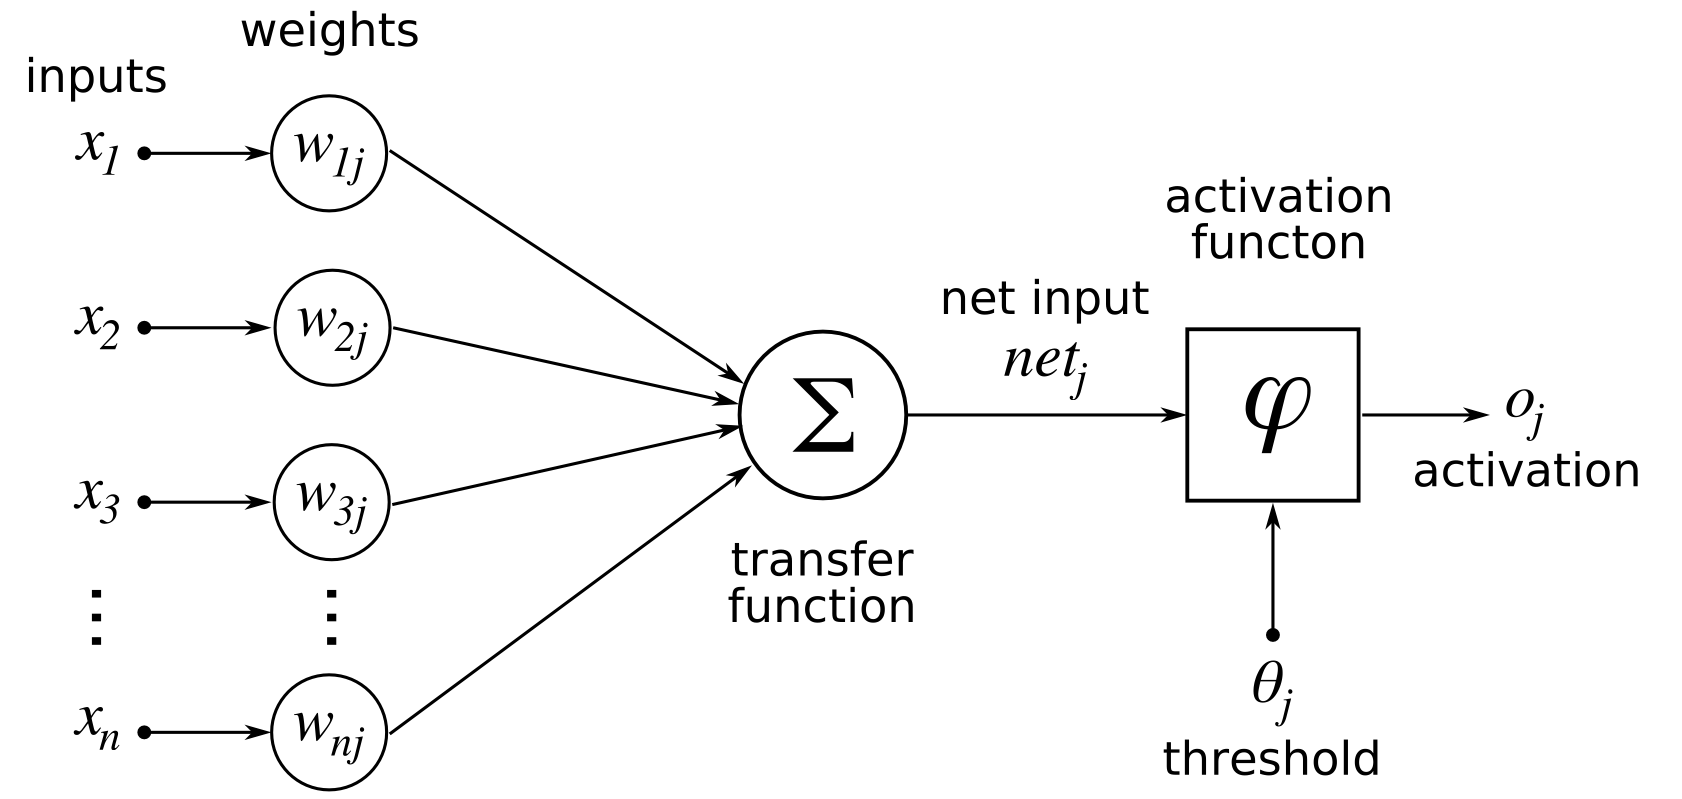
\includegraphics[width=.7\textwidth]{images/ArtificialNeuronModel}} 
	\caption{Artificial Neuron Model}
	\label{fig:Modello matematico di un neurone artificiale}
\end{figure}

\subsection{Funzioni di attivazione}
\label{subsec:fattivazione}
Una funzione di attivazione è una componente fondamentale del modello. Essa consente alla rete di imparare trasformazioni non lineari, in modo da essere in grado di calcolare problemi non banali utilizzando un limitato numero di nodi.

Una delle funzioni più utilizzate è la \emph{sigmoide} $\sigma(x)$, la quale modella la frequenza degli stimoli emessi, da neurone inattivo, $\sigma(x)=0$, a neurone completamente saturo con una frequenza di attivazione massima, $\sigma(x)=1$.

\begin{equation}
\sigma(x) = \frac{1}{1+e^{-x}}
\label{eq:sigmoid}
\end{equation}


Negli ultimi anni è diventata molto popolare la \emph{Rectified Linear Unit} (ReLU) \cite{nair2010rectified,hahnloser2000digital,hahnloser2003permitted,glorot2011deep}, definita dalla seguente equazione:
\begin{equation}
f (x) = \max(0, x)= \begin{cases}
x \quad \mbox{se } x>0\\
0 \quad \mbox{altrimenti}
\end{cases}
\label{eq:relu}
\end{equation}
Questa funzione azzera tutti i valori negativi, mentre ritorna invariati quelli positivi.

Essa viene utilizzata per la sua capacità di accelerare notevolmente il processo di ottimizzazione, inoltre la sua implementazione risulta semplice ed efficiente.

\begin{figure}[htb]
	\centering
	\subfloat[][\emph{Sigmoide}]
	{\includegraphics[width=.45\textwidth]{images/signmoid2}}
	\quad
	\subfloat[][\emph{ReLU}]
	{\includegraphics[width=.45\textwidth]{images/relu2}} 
	
	\caption{Andamento di due funzioni di attivazione}
	\label{fig:subfig}
\end{figure}

\section{Architetture}
\label{sec:architetture}

I neuroni vengono organizzati in una struttura detta architettura della rete.
I dati, partendo da un livello iniziale, chiamato layer di input, attraversano i multipli strati interni della rete, gli hidden layer, raggiungendo l'ultimo livello detto layer di output.

Quando i collegamenti tra i neuroni formano una struttura senza cicli si parla di reti \emph{feed-forward} \cite{svozil1997introduction}.

\subsection{Layer fully-connected}
\label{subsec:fc}

Un’architettura molto comune nelle reti neurali è una struttura ``densa'', che utilizza \emph{layer fully-connected}, in cui tutti i neuroni del livello precedente sono collegati ad ogni neurone dello strato successivo \cite{sainath2015convolutional}.

Lo scopo di un layer completamente connesso è imparare combinazioni non lineari di feature ad alto livello provenienti dal layer precedente. 
Una struttura di questo tipo è però caratterizzata da un numero di connessioni che cresce molto velocemente, causando un accrescimento del numero di parametri che la rete deve apprendere.
Questo comporta un aumento del costo computazionale e un alto rischio di overfitting, approfondito nella sezione \ref{subsec:overfitting}.

Per questo motivo questi vengono spesso sostituiti dai layer convoluzionali.

\subsection{Layer convoluzionali}
\label{subsec:cnn}
Una rete neurale convoluzionale, in inglese \emph{Convolutional Neural Network} (CNN), è una classe di reti artificiali avanzate e \emph{feed-forward}, composte da uno o più strati convoluzionali seguiti da una serie di livelli completamente connessi \cite{kim2014convolutional}.

Una convoluzione può essere considerata come una funzione a finestra scorrevole, detta \emph{kernel} o filtro, applicata a una matrice. 
Ogni livello applica filtri diversi, in genere centinaia o migliaia, e combina i loro risultati. 
Durante la fase di addestramento, una CNN impara automaticamente i valori dei suoi filtri in base all'attività che si desidera eseguire. 


Due parametri che definiscono il comportamento di un layer convoluzionale sono lo \emph{stride}, che rappresenta il passo di 
convoluzione e viene utilizzato per ridurre le dimensioni spaziali dell'output e il \emph{padding}, che definisce il comportamento dei neuroni lungo 
i bordi dei dati di input. Se viene scelto un padding \emph{valid}, l'output contiene solo i neuroni la cui regione di convoluzione è completamente contenuta nei dati; nel caso di padding \emph{same}, invece, l'output mantiene la stessa dimensione dell'input, utilizzando zero come valore per i dati mancanti.

Le reti convoluzionali sono adatte per elaborare dati visivi e altri dati bidimensionali, ed hanno mostrato ottimi risultati nel riconoscimento di immagini e nella manipolazione del linguaggio naturale \cite{manning1999foundations}.
In quest'ultimo caso, l'input è costituito da frasi o documenti rappresentati come una matrice, in cui ogni riga corrisponde a un token, in genere una parola. Tipicamente, questi vettori sono dei word embeddings (rappresentazioni a bassa dimensione) come word2vec \cite{mikolov2013distributed}, ma potrebbero anche essere vettori unici che indicizzano la parola in un vocabolario. 

Nel \emph{Natural Language Processing} (NLP) utilizziamo filtri che scorrono su righe complete della matrice (parole), pertanto, la loro ``larghezza'' è solitamente uguale alla quella della matrice di input. L'altezza, o la dimensione della regione, può variare, ma le finestre tipicamente scorrono su 2-5 parole per volta. 

Risulta che le CNN applicate ai problemi di NLP funzionino abbastanza bene, un esempio è il modello \emph{bag-of-words} che è stato l'approccio standard per anni e ha portato a risultati piuttosto buoni \cite{wallach2006topic}.

Le CNN sono più facili da addestrare e hanno molti meno parametri da stimare. 
Il minor numero di connessioni e pesi di questa architettura, rende gli strati convoluzionali relativamente economici in termini di memoria e potenza di calcolo necessari.

\subsection{Layer di pooling}
\label{subsec:maxpool}

Il \emph{pooling} è un processo alquanto comune nelle reti neurali, la cui funzione è ridurre progressivamente la dimensionalità spaziale per diminuire la quantità di parametri e la complessità computazionale della rete, mantenendo le informazioni più salienti e controllando anche l'overfitting.

Il layer di pooling opera indipendentemente su ogni slice di profondità dell'input e lo ridimensiona spazialmente, usando l'operazione MAX sul risultato di ogni filtro \cite{karpathy2016cs231n}. 

Una proprietà del pool è che fornisce una matrice di output a dimensione fissa --- in genere richiesta per la classificazione. Ciò consente di utilizzare frasi di dimensioni variabili e filtri di dimensioni variabili, ma ottenere sempre le stesse dimensioni di output da inserire in un classificatore.

\subsection{Batch Normalization}
\label{subsec:normalization}

Durante la fase di addestramento del modello, i parametri di ogni substrato vengono ottimizzati al fine di minimizzare l'errore finale.
Ad ogni iterazione, in ciascuno strato avviene una variazione dell'output, corrispondente ad una variazione nei valori in ingresso al livello successivo.
Questo può rappresentare un problema per la rete, che deve adattare i propri strati ad un continuo cambiamento nell'input. 

Per aumentare la stabilità della rete neurale, velocizzare il training e migliorarne le performance, generalmente viene applicata ad ogni strato una \emph{Batch Normalization}  \cite{ioffe2015batch}, la quale normalizza l'uscita di un precedente livello sottraendo il valore medio di un batch e dividendo il risultato per la sua deviazione standard.
\begin{equation}
	\hat{x}^{(k)}=\frac{x^{(k)}-\mean[x^{(k)}]}{\sqrt{\variance[x^{(k)}]}}
\end{equation}

L'applicazione di questa operazione ad ogni input potrebbe cambiare ciò che il layer può rappresentare. Per questo motivo viene assicurato che la trasformazione inserita nella rete possa rappresentare l'identità, in modo da poter annullare il potenziale effetto della Batch Normalization, nel caso in cui fosse l'azione ottimale.
Dunque viene prevista l'aggiunta di due parametri --- ``deviazione standard'' $\gamma$ e ``media'' $\beta$ --- che la rete impara assieme ai parametri del modello originale, come mostrato nell'equazione \ref{eq:batchnorm}
\begin{equation}
	y^{(k)}=\gamma^{(k)}\hat{x}^{(k)}+\beta^{(k)}\mbox{.}
	\label{eq:batchnorm}
\end{equation}

La \emph{Batch Normalization} può essere utilizzata sia su reti \emph{feed-forward}, sia sulle \emph{reti convoluzionali}.
In questo secondo caso, media e varianza vengono calcolate per ogni filtro.

\section{Apprendimento}
\label{sec:apprendimento}
Per insegnare alla rete a risolvere un determinato problema, occorre una fase di addestramento in cui vengono condotte una serie di osservazioni per stabilire quali valori assegnare ad ogni parametro della rete e trovare un modello ottimale.

Questo processo di apprendimento viene strutturato come un problema di ottimizzazione in cui lo scopo è minimizzare una \emph{funzione di costo}, che misura la distanza tra una soluzione particolare ed una ottima. 

\subsection{Funzione di costo}
\label{subsec:loss}

Una funzione di costo mappa un evento ad un numero reale, il quale ne rappresenta intuitivamente il ``costo''.

Nella strategia adottata si utilizzeranno due diverse funzioni obiettivo: l'\emph{errore quadratico medio} per risolvere il problema di regressione, e la \emph{Softmax Cross Entropy} per il compito di classificazione. Mentre per la costruzione dell'embedding verrà applicata la \emph{Noise Contrastive estimation}.

\subsubsection{Mean Squared Error}
\label{subsubsec:MSE}

Per il task il cui compito è prevedere dei valori reali è comune calcolare lo scostamento tra la quantità prevista dalla rete $(\hat{Y})$ e i valori osservati $Y$ (ground truth). 
 
L'\emph{errore quadratico medio} (MSE) di uno stimatore misura la media dei quadrati degli errori, e viene calcolato come

\begin{equation}
\mse = \frac{1}{n}\sum_{i=1}^{n}(Y_i-\hat{Y}_i)^2 \mbox{.}
\end{equation}

con $n$ numero delle previsioni \cite{wang2009mean}.

\subsubsection{Softmax Cross Entropy}
\label{subsubsec:sce}

Softmax è una funzione di loss comunemente utilizzata per la classificazione. In particolare viene applicata allo strato finale della rete ed addestrata in un regime di entropia incrociata \cite{tang2013deep}.\\
L'entropia incrociata è un indicatore che può essere utilizzato per misurare l'accuratezza delle previsioni. 

Date due variabili casuali discrete $p$ e $q$ definiamo l'entropia nel modo seguente:
\begin{equation}
	H(p,q)=-\sum_{x} p(x) \log q(x)
\end{equation}

in cui $p_{x}$ è la ``vera'' probabilità o distribuzione, mentre $q_{x}$ è la distribuzione ``innaturale'' ottenuta a partire dal modello corrente.

Nella pratica la \emph{Cross Entropy} viene calcolata empiricamente ipotizzando l'equiprobabilità degli eventi, poiché $p$ è ignota. 
Di conseguenza, è ridefinibile come segue

\begin{equation}
H(q)=-\frac{1}{N}\sum_{x} \log q(x)
\end{equation}

dove N è il numero di eventi osservati.

L'obiettivo principale di questa funzione è rendere il risultato della Softmax campionata uguale a quella vera. L'algoritmo si concentra sulla selezione di campioni specifici dalla distribuzione data per ottenere la loss desiderata \cite{liu2016large}.  
L'utilizzo della funzione Softmax ha un effetto considerevole sulle prestazioni. 

\subsubsection{Noise Contrastive estimation}
\label{subsubsec:nce}

La stima contrastiva del rumore è una strategia utilizzata nell'ambito della modellazione linguistica o per la generazione di word embedding dati in input dei corpus molto ampi.

La funzione obiettivo del modello \emph{skip-gram} cerca di trovare rappresentazioni di parole che siano utili per predire le parole circostanti, meglio chiamati contesti, in una frase o in un documento. 
Data una sequenza di parole di addestramento, la funzione obiettivo massimizza la probabilità media di log
\begin{equation}
\frac{1}{T}\sum_{t=1}^{T} \sum_{-c \leq j \leq c, j \neq 0} \log p(w_{t+j} | w_T)
\end{equation}

dove $c$ è la dimensione del contesto di training \cite{mikolov2013distributed}. 

Nell'implementazione del modello \texttt{word2vec}, la formulazione standard dello \emph{skip-gram} definisce la precedente probabilità di log ricorrendo alla funzione Softmax:
\begin{equation}
p_{\theta}(w_{O} | w_{I}) = \frac{\exp({v^{\prime}_{w_{O}}}^{\top} v_{w_{I}})}{\sum_{w=1}^{W} \exp({v^{\prime}_{w}}^{\top} v_{w_I})}
\end{equation}

dove $v_w$ e $v'_w$ sono le rappresentazione vettoriali di input e output e $W$ è il numero delle parole del vocabolario \cite{dyer2014notes}.

In questo modo la previsione di una data parola a partire da un contesto risulta essere un compito computazionalmente intenso, poiché vi sono operazione che coinvolgono l'intero dizionario.

Di conseguenza, un alternativa alla funzione Softmax è l'applicazione della \emph{Noise Contrastive estimation} con campionamento negativo \cite{liu2016classification, viswesvaran2000measurement}. Essa consente un allenamento più veloce e rappresentazioni vettoriali migliori per le parole frequenti.

\subsection{Algoritmi di ottimizzazione}
\label{subsec:optimizer}

Gli algoritmi di ottimizzazione sono necessari per minimizzare il risultato di una determinata funzione obiettivo, la quale dipende dai parametri che il modello deve imparare durante l'addestramento. 

Vengono utilizzate varie strategie e algoritmi di ottimizzazione per aggiornare e calcolare i valori appropriati e ottimali di tale modello, i quali influenzano fortemente l'efficacia del processo di apprendimento.

L'entità dell'aggiornamento è determinata dal tasso di apprendimento $\eta$, in inglese \emph{learning rate}, che garantisce la convergenza al minimo globale, per superfici di errore convesse, e ad un minimo locale, per superfici non convesse. 

\subsubsection{Stochastic Gradient Descent}
\label{subsubsec:SGD}

La discesa del gradiente, in inglese \emph{Gradient Descent} (GD), è un algoritmo iterativo per l'ottimizzazione di funzioni \cite{ruder2016overview}.

Viene utilizzato principalmente per eseguire gli aggiornamenti dei pesi in un modello di rete neurale nel seguente modo
\begin{equation}
\theta = \theta - \eta \nabla J(\theta)
\end{equation}
dove $\eta$ rappresenta il tasso di apprendimento, $\nabla J(\theta)$ è il gradiente della funzione di loss $J(\theta)$ rispetto al parametro $\theta$. 

La tradizionale discesa gradiente, o \emph{Batch Gradient Descent} (GD), calcola il gradiente dell'intero set di dati, eseguendo un solo aggiornamento. Di conseguenza il processo di addestramento può risultare lento e difficile da controllare per i set di dati che sono molto grandi. 

I problemi che si verificano con questo algoritmo vengono risolti applicando una sua variante: la {discesa stocastica del gradiente}, in inglese \emph{Stochastic Gradient Descent} (SGD).
Questa tecnica esegue un aggiornamento alla volta dei parametri per ognuno degli esempi di training
\begin{equation}
\theta = \theta - \eta \nabla J(\theta; x(i); y(i))
\end{equation}

dove $x(i)$ e $y(i)$ sono le coppie di esempi usati per l'addestramento.

Questa tecnica risulta essere molto più veloce di quella classica. 
A causa dei frequenti aggiornamenti, i parametri presentano un'alta varianza, inoltre la funzione loss oscilla tra diverse intensità. Questo favorisce la scoperta di nuovi minimi locali, complicando però la convergenza all'ottimo globale. 


\subsubsection{Adagrad}
\label{subsubsec:adagrad}

\emph{Adagrad} è un metodo di apprendimento adattativo che aggiusta il learning rate sulla base dei parametri \cite{duchi2011adaptive} .
In questo algoritmo, la dimensione degli aggiornamenti è grande per parametri associati a caratteristiche poco ricorrenti e piccola per quelli più frequenti. Per questo motivo viene considerato adatto alla gestione di dati sparsi.

Adagrad modifica il tasso di apprendimento generale $\eta$ ad ogni istante di tempo $t$ per ogni parametro $\theta(i)$, sulla base dei gradienti che sono stati calcolati per $\theta(i)$.

Il vantaggio principale di questo metodo è che non è necessario regolare manualmente la frequenza di apprendimento e nella maggior parte delle implementazioni viene usato un valore predefinito --- per esempio \numprint{0,001} --- e lasciato invariato.\\
La principale debolezza consiste nell'accumulo dei ``gradienti quadrati'' nel denominatore, finché ogni termine aggiunto è positivo \cite{ruder2016overview}. Di conseguenza il tasso di apprendimento si riduce fino al punto in cui l'algoritmo non è più in grado di acquisire ulteriori conoscenze. 

\subsection{Paradigmi di apprendimento}
\label{subsec:Paradigmi di apprendimento}

Gli algoritmi di apprendimento sono principalmente suddivisi in due categorie:
\begin{itemize}
	\item[\bfseries supervisionato] --- alla rete viene presentato un training set preparato da un ``insegnante esterno'', composto da coppie significative di valori (input, output atteso).
	
	Quando alla rete neurale viene fornito l'input dall'ambiente, l'insegnante calcola l'output desiderato corrispondente, addestrando la rete mediante un algoritmo (tipicamente quello di back propagation \cite{horikawa1992fuzzy}). 
	
	La rete impara a riconoscere la relazione incognita che lega le variabili di ingresso e uscita, in modo da prevedere il valore di output per qualsiasi valore di ingresso, basandosi solo su una casistica di corrispondenze (coppie input-output).
	
	\item[\bfseries non supervisionato] --- alla rete vengono presentati solo i valori di input, mentre non sono messe a disposizione le informazioni di ritorno dell'ambiente sui valori obiettivo che si vogliono ottenere in risposta o riguardo la correttezza dell'output fornito.
	
	La rete è in grado di individuare da sola pattern, caratteristiche, similarità e regolarità statistiche nei dati di input, acquisendo la capacità di dividerli in cluster rappresentativi che sviluppino delle rappresentazioni interne, senza usare confronti con output noti.
	
	In questo caso, gli algoritmi che modificano i pesi della rete fanno riferimento solo ai dati contenuti nelle variabili di ingresso.
	
	Questo è un tipo di apprendimento autonomo senza controllo esterno sull'errore. È un approccio adatto per ottimizzare le risorse nel caso in cui non si conoscano a priori i gruppi in cui dividere l'input.
\end{itemize}

\section{Train, Validation e Test Sets}
\label{sec:set}
Per misurare le prestazioni di una rete neurale dopo la fase di apprendimento, viene creato un test set formato da coppie non utilizzate per il training e validation set.\\
Vengono generalmente definiti: 
\begin{itemize}
	\item Training set --- sul quale viene eseguito l'algoritmo di apprendimento.
	\item Validation set --- viene utilizzato per regolare i parametri, selezionare le features e prendere decisioni per quanto riguarda l'algoritmo di apprendimento.
	\item Test set --- si utilizza per valutare le performance dell'algoritmo, ma non per prendere decisioni su quale algoritmo di apprendimento o parametri utilizzare. 
\end{itemize}

Una volta definiti i set, ci si concentrerà sul miglioramento delle prestazioni del training e validation set. 

Generalmente la dimensione del test set è un terzo di quella del training. Esso è composto da input critici su cui la risposta della rete deve essere buona. 
Questo funziona bene quando sono messi a disposizione un numero limitato di esempi, ma nell'era dei Big Data, dove i problemi di apprendimento automatico consistono di più di un miliardo di campioni, la frazione di dati allocati agli insiemi di sviluppo e test è ridotta, nonostante il valore assoluto di esempi sia maggiore.

Vengono utilizzate diverse tecniche statistiche per valutare la bontà di un modello.

\subsection{Evaluation metric}
\label{subsec:EvaluationMetric}

Le metriche di valutazione misurano le prestazioni di un modello, discriminando la bontà dei risultati ottenuti.
Vengono presi in considerazione diversi tipi di metriche per valutare i modelli. La scelta della metrica dipende completamente dal tipo di modello e dal piano di implementazione. 

I modelli predittivi si distinguo in due principali categorie: si parla di \emph{regressione} quando l'output da prevedere è continuo, o di \emph{classificazione} nel caso in cui l'output sia nominale o binario. 
\subsubsection{Regressione}
\label{subsubsec:regressione}

L'{scarto quadratico medio}, in inglese \emph{Root Mean Squared Error} (RMSE), è la metrica di valutazione più popolare utilizzata nei problemi di regressione. Questo parametro aiuta a fornire risultati affidabili, mostrando correttamente la grandezza del termine di errore.
La metrica RMSE è definita dalla seguente equazione
\begin{equation}
	\rmse = \sqrt{\frac{\sum_{i=1}^{N}({Y}_i - \hat{Y}_i)^2}{N}} \mbox{.}
	\label{eq:rmse}
\end{equation}

con $\hat{Y}$ quantità prevista dalla rete, $Y$ i valori osservati e $N$ numero delle previsioni.
\subsubsection{Classificazione}
\label{subsubsec:classificazione}

Nei problemi di classificazione, in particolare quella binaria, gli output sono 0 o 1. \\
Una \emph{matrice di confusione}, nota anche come matrice di errore, è una tabella $2 \times 2$, generalizzabile ad una $N \times N$ per problemi ad $N$ classi, che consente la visualizzazione delle prestazioni di un algoritmo di apprendimento supervisionato. 

Ogni colonna della matrice rappresenta le istanze previste di una classe mentre ciascuna riga quelle osservate. 

\begin{figure}[t]
	\centering
	{\includegraphics[width=.3\textwidth]{images/confmatrix}}
	\caption{Visualizzazione di una matrice di confusione}
	\label{fig:confmat}
\end{figure}

L'individuazione di falsi positivi (casi negativi identificati come positivi), falsi negativi (casi positivi identificati come negativi), veri positivi (casi positivi correttamente identificati) e veri negativi (casi negativi correttamente identificati), mostrati nella figura \ref{fig:confmat}, consentono  un'analisi più dettagliata della semplice proporzione di classificazioni corrette.

È possibile estrarre da questa tabella le seguenti misure di performance:
\begin{itemize}
	\item l'\emph{accuracy}, o accuratezza, del modello, che consiste nella porzione rispetto al totale delle previsioni corrette
	\begin{equation}
		\frac{\mbox{True Positive} + \mbox{True Negative}}{\mbox{True Positive} + \mbox{True Negative} + \mbox{False Positive} + \mbox{False Negative}}
	\end{equation} 
	\item la \emph{precision}, o precisione, cioè la porzione dei casi positivi identificati correttamente
		\begin{equation}
	\frac{\mbox{True Positive}}{\mbox{True Positive} + \mbox{False Positive}}
	\end{equation}
	
	\item la \emph{recall}, ovvero la porzione dei casi positivi reali correttamente identificati
		\begin{equation}
	\frac{\mbox{True Positive}}{\mbox{True Positive} + \mbox{False Negative}}
	\end{equation}
\end{itemize}


\subsection{Overfitting}
\label{subsec:overfitting}

L'\emph{overfitting} è ``la produzione di un'analisi che corrisponde esattamente a un particolare insieme di dati o ne presenta forti similarità; può determinare l'impossibilità di adattamento a nuovi dati o compromettere l'affidabilità delle predizioni sulle osservazioni future''.

La rete neurale deve avere la capacità di comprensione del modello statistico dei dati. In presenza di overfitting essa memorizza i dati del training set e non è quindi in grado di generalizzare su nuovi dati. L'essenza di questo problema consiste nell'estrarre inconsapevolmente parte della variazione residua (cioè il rumore) come se quella variazione rappresentasse la sottostante struttura del modello \cite{burnham2003model}.

Per ridurre la possibilità di overfitting esistono diverse tecniche, come la convalida incrociata (Cross Validation), la regolarizzazione o l'\emph{early stopping}, che consiste nell'utilizzo di un validation set di coppie non usate nel training set per la misurazione dell'errore.

\include{chap_quo}
\include{chap_qua}

\appendix
% INCLUSIONE APPENDICI -
\include{app_a}

%%%%%%%%%%%%%%%%%%%%%%%%%%%%%%%%%%%%%%%%%%%%%%%%%%%%%%%%%%%%%%%

% BIBLIOGRAFIA
\addcontentsline{toc}{chapter}{\refname}
\nocite{*}
\printbibliography

\end{document}